%!TEX root = ../../../adrien_gomar_phd.tex
\chapter{11\texorpdfstring{\textsuperscript{th}}{th} standard aeroelastic configuration}
\label{cha:stcf11}

\defcitealias{Sicot2014}{{\small F. Sicot, \emph{A. Gomar}, G. Dufour and A. Dugeai. 
Time-Domain Harmonic Balance Method for Turbomachinery Aeroelasticity.
\emph{AIAA Journal}, 52(1):62--71, January 2014}}

\chabstract{The harmonic balance method along with a aeroelastic 
weak-coupling approach, is applied to
the well-known 11\textsuperscript{th} standard aeroelastic configuration of
\citet{Fransson1999} is used. It is shown that by using only
one harmonic ($N=1$), the damping curve of both the subsonic
and the transonic operating points are superimposed on
the reference unsteady computation. The agreement
with both the experimental and the numerical data available
is good, justifying the proposed approach. Moreover, a
speed-up of seven is found compared to a classical 
time-marching scheme. This work has been published in
\begin{quote}
	\citetalias{Sicot2014}
\end{quote}}


\newpage

\section{Presentation of the case}
\label{sec:stcf11_presentation}
%!TEX root = ../../../adrien_gomar_phd.tex

For external-flow aeroelasticity, the HB approach has 
been thoroughly validated by \citet{Gopinath2005, Woodgate2009} and \citet{JDufour2009}, 
mostly for the AGARD test cases of \citet{Davis1982}.
Experimental data for turbomachinery aeroelasticity are more scarce: 
the STandard aeroelastic ConFigurations (STCF) experiments 
of \citet{Fransson1999} are the 
reference in this respect, and have been widely used 
to validate different numerical approaches by \citet{Sbardella2001,
Duta2002,Campobasso2003,Cinnella2004} and \citet{Huang2013a} whose
uses a similar harmonic balance approach as the one proposed in
this work.
The experiments
are composed of 11~turbomachinery configurations that have been
thoroughly investigated experimentally in an 
annular test rig at \'Ecole 
Polytechnique F\'ed\'erale de Lausanne.

In particular, the 11\textsuperscript{th} standard configuration is a
turbine stator composed of 20~blades, and tested
in the late 1990's by \citet{Fransson1999}.
The experimental results have been found to be highly reproducible and
therefore suitable for code validation.  Moreover,
two flow regimes are considered, one subsonic and one transonic.
In this respect, the transonic case allows to distinguish
solvers able to capture non-linear unsteady effects. This is why this particular
case is used here, since HB methods are meant to capture non-linear unsteady
features. However, it must be pointed out that LUR approaches have
been validated using the transonic case and show fair agreement with experimental
data~\cite{Sbardella2001, Duta2002,Campobasso2003}.

% geometry presentation
The geometry profile and the results are available over the
internet~\cite{stcf11web}. 
To characterize the two flow regimes, measurements of static and total pressures 
as well as flow angles are done in two planes $e_0$ located $0.3$ axial chord upstream 
of the turbine
blade and $e_1$ located $0.6$ axial chord downstream
as shown in Figure~\ref{fig:stcf11_measurements}.
\begin{figure}[htp]
  \centering
  \includegraphics*[width=0.40\textwidth]{stcf11_measurements.pdf}
  \caption{Position of the measurement planes in the STCF~11 configuration.}
  \label{fig:stcf11_measurements}
\end{figure}
The results are given in terms of
inlet Mach number $M_0$, inlet total pressure $p_{i_0}$, 
inlet flow angle $\beta_0$, outlet isentropic
Mach number $M_{1_{is}}$ and outlet static pressure $p_{s_1}$. 
The isentropic Mach number is the Mach number 
computed if the stagnation pressure was taken constant (without loss)
\begin{equation}
    M_{is} = \sqrt{\frac{2}{\gamma -1}
        \left[\left( \frac{p_{i_0}}{p_s} \right)^{\frac{\gamma - 1}{\gamma}}  
        - 1 \right]},
\end{equation}
where $p_{i_0}$ is the constant total pressure and $p_s$
the local static pressure.
It is actually
one way to interpret the static pressure as a velocity.
The experimental results measured at plane $e_0$
and $e_1$ are given in Tab.~\ref{tab:stcf11_steady_results}. 
These will be used later on to set the boundary conditions 
of the CFD computations. To allow local validation of the steady
flow, the experimental results of 
isentropic Mach number are given at blade wall.
\begin{table}[htp]
  \ra{1.3} \centering
  \begin{tabular}{lccccc}
    \toprule
    \phantom{abdefghijk}& $M_0~[-]$ & $p_{i_0}~[\text{Pa}]$ & $\beta_0~[\circ]$ & $M_{1_{is}}~[-]$ & $p_{s_1}~[\text{Pa}]$ \\
    \midrule
    Subsonic & $0.31$ & $124,600$ & $15.2$ & $0.69$  & $90,700$ \\
    Transonic & $0.4$ & $229,800$ & $34$    & $0.99$ & $122,400$ \\
    \bottomrule
  \end{tabular}
  \caption{Steady experimental results for the STCF~11 configuration.}
  \label{tab:stcf11_steady_results}
\end{table} 

For aeroelastic investigations, the blades oscillate harmonically in the first bending mode
at a reduced frequency of $f_{c} =\pi c f/U_{outlet, exp} = 0.2134$ 
for the subsonic case and $0.1549$ for the
transonic case. Aeroelastic
results are available such as the first harmonic of the unsteady pressure
coefficient at blade walls (amplitude and phase), for several nodal
diameters. These are measured using piezo-resistive pressure transducers.

The damping is evaluated at blade walls through through the
expression given by~\citet{Fransson1999}
\begin{equation}
    \delta [-] = - \sum^{\#~pts}_{k=0} \frac{c}{h} 
      \frac{|\widehat{p}_k|}{(p_{i_0} - p_{s_0})} S_k \arg (\widehat{p}_k),
\end{equation}
where $c$ is the chord length,
$h$ the bending amplitude, $| \widehat{p} |$ 
and $\arg (\widehat{p})$ are the modulus and the phase of the
complex first harmonic of static pressure, respectively, $S$ the surface
and $k$ denotes the k\textsuperscript{th}
grid point at blade walls.
The damping strongly varies under small changes in the
local distribution. It is therefore recommended to look at the local
distributions. No experimental damping curves are given. In fact,
there is too few measurement points to integrate the results with
confidence. However, \citet{Fransson1999}
provide numerical results of the damping curve obtained with a potential code.



\section{Numerical setup}
\label{sec:stcf11_numerical}
%!TEX root = ../../../adrien_gomar_phd.tex

% mesh presentation
The blade passage is meshed using an O4H 
topology as shown in Fig.~\ref{fig:stcf11_mesh}.
The number of grid points along the blade
chord axis is~160 and the computed $y^+$ at the walls is $\mathcal{O}(1)$.
The blade has the same profile along the spanwise direction and no
twist. Therefore, a 2.5D mesh is used with five points 
in the radial direction, with a spanwise
extent representing $1\%$ of the chord. 
81 points are used to discretize the azimuthal direction.
The total size of the mesh is 70330.
\begin{figure}[htb]
  \centering
  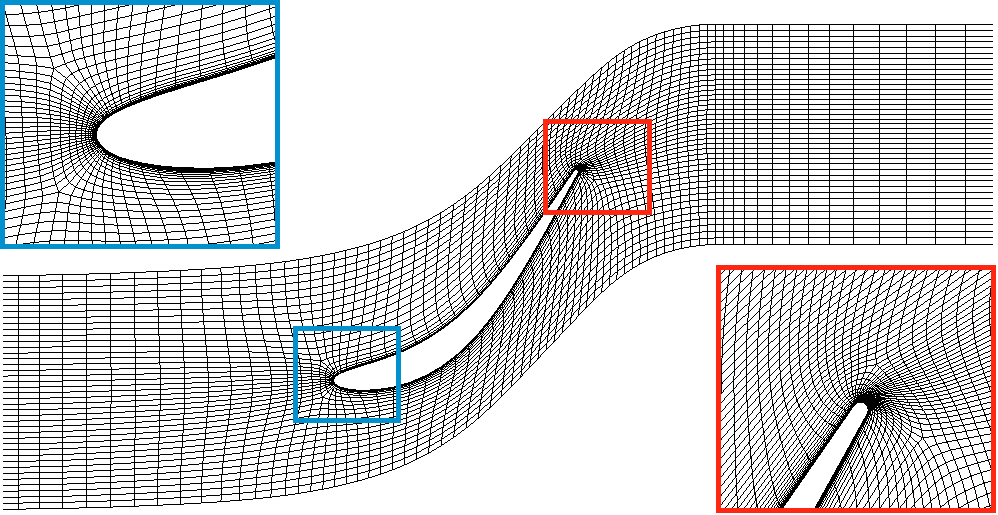
\includegraphics[width=.46\linewidth]{STCF11_MESH.pdf}
  \caption{STCF 11 mesh}
  \label{fig:stcf11_mesh}
\end{figure}

% boundary conditions
The boundary conditions used for this case are: (i)~an
injection condition  for the inlet (with a relative flow angle
set to the  experimental value using Tab.~\ref{tab:stcf11_steady_results}), 
(ii)~a constant static pressure
condition for the outlet using also Tab.~\ref{tab:stcf11_steady_results},  
(iii)~an adiabatic no-slip condition on
blade walls, and (iv)~periodic or phase-lagged conditions 
for azimuthal boundaries depending on the  
prescribed IBPA.

% numerical parameters
Turbulence is modeled using the one-equation model of
\citet{Spalart1992}.  The third-order upwind \citet{Roe1981}
scheme is used to compute the convective fluxes.
The maximum
CFL number is set to~20 for the steady computations,  the inner loop
of the DTS scheme and the HB simulations.  For the DTS scheme,  
convergence in time discretization is obtained
after 20~periods using 128~instants per period.  Iterative convergence 
for the inner loop is considered achieved when the normalized
residuals drop by $5\cdot 10^{-2}$ (within a maximum of
50~sub-iterations).

\subsection{Influence of the mesh discretization}
\label{sub:stcf11_mesh_convergence}
The mesh quality is assessed through both the $y^+$
at the walls that is $\mathcal{O}(1)$ and a mesh convergence.
To ensure this last, three meshes are tested, the referenced one
described above, and two meshes, coarsen~2 and coarsen~4,
coarsened by a factor two and four in each directions respectively.
The steady results for the two operating points are shown 
in Fig.~\ref{fig:stcf11_mesh_convergence}.
\begin{figure}[htb]
  \centering
  \subfigure[Subsonic]{
    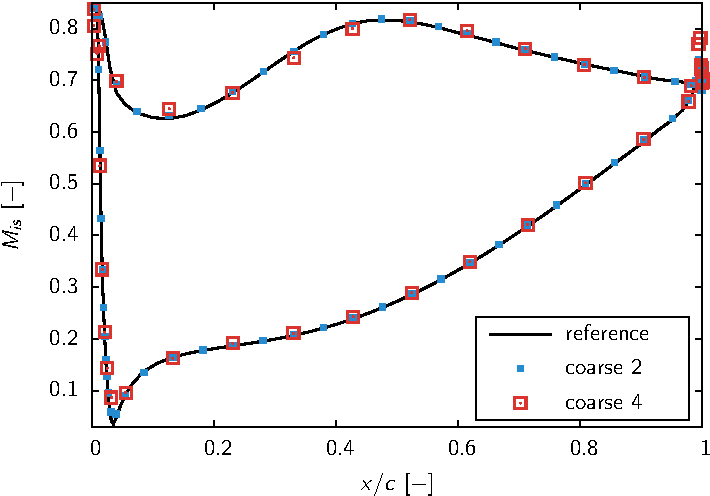
\includegraphics[width=.4\textwidth]{STCF11_RANS_SUBSONIC_CONVERGENCE_MESH_PPT.pdf}}
  \subfigure[Transonic]{
    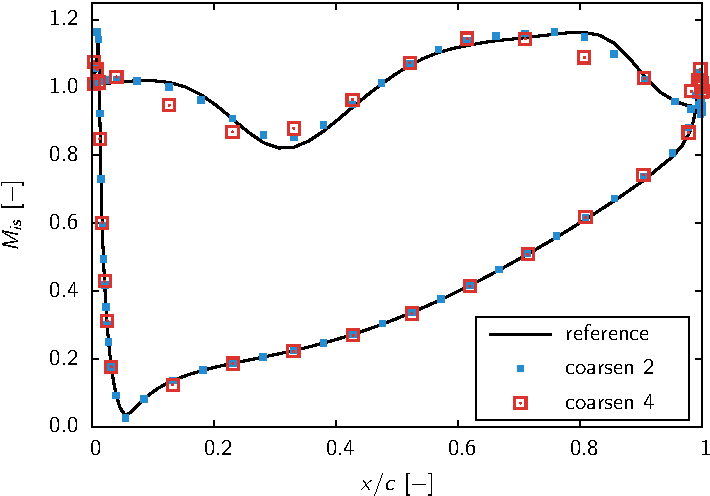
\includegraphics[width=.4\textwidth]{STCF11_RANS_TRANSONIC_CONVERGENCE_MESH_PPT.pdf}}
  \caption{Influence of mesh discretization for the STCF~11 configuration.}
  \label{fig:stcf11_mesh_convergence}
\end{figure}
The three meshes give the same results for the subsonic case. On the
pressure side (bottom curve), the three results are superimposed. On the suction side
(top curve),
some minor differences are observed in particular near
$x_c \leq 0.2$. Nevertheless, the agreement
between the three meshes is very good for the subsonic operating point.
The results are more scattered for the transonic operating point. In fact,
the coarsen~4 mesh does not accurately predict the region where $x_c \leq 0.3$
and where $0.5 \leq x_c \leq 0.8$. This last zone seems smeared out. 
However, the results
obtained with the coarsen~2 mesh are in good agreement with the referenced mesh.
Therefore, the reference mesh is retained for the following study.

\subsection{Influence of the spatial discretization}
To assess the influence of spatial discretization, four space schemes are
used to compute both the subsonic and transonic steady field. These
four schemes are the \citet{Jameson1981} scheme (noted JST) with $\kappa_4 = 0.016$
and $\kappa_2$ equal to $0.5$ and $1.0$ for respectively the subsonic and the transonic
inflow conditions. In addition to this scheme, three \citet{Roe1981} schemes are used,
a theoretical third order with no limiter (noted Roe~3), a second order limiter~\cite{Roe1981} (noted Roe~2)
and a first order limiter (noted Roe~1).
The steady results for the two operating points are shown 
in Fig.~\ref{fig:stcf11_space_scheme_convergence}.
\begin{figure}[htb]
  \centering
  \subfigure[Subsonic]{
    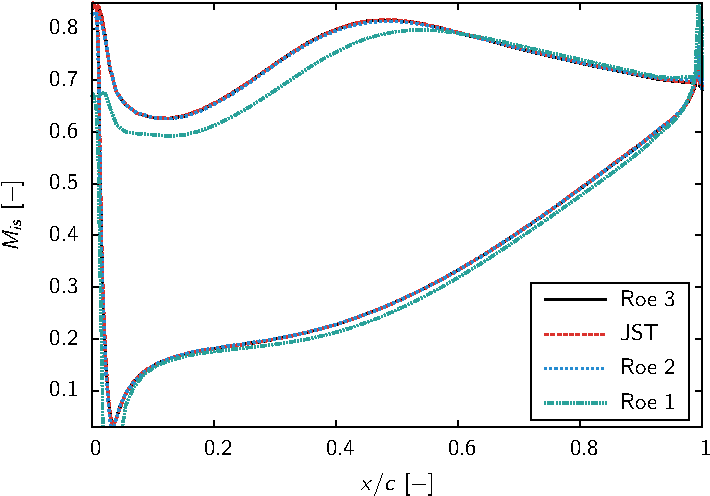
\includegraphics[width=.4\textwidth]{STCF11_RANS_SUBSONIC_SPACE_SCHEME_PPT.pdf}}
  \subfigure[Transonic]{
    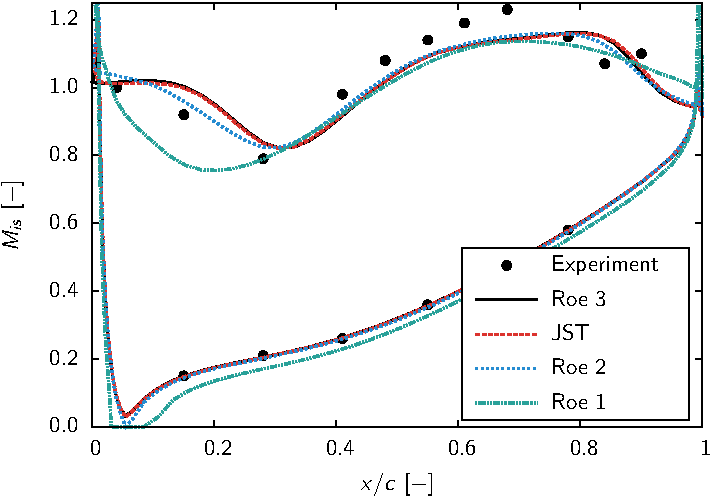
\includegraphics[width=.4\textwidth]{STCF11_RANS_TRANSONIC_SPACE_SCHEME_PPT.pdf}}
  \caption{Influence of mesh discretization for the STCF~11 configuration.}
  \label{fig:stcf11_space_scheme_convergence}
\end{figure}
For the subsonic case, the results are all superimposed except for the first 
order limiter Roe scheme. This was expected as first order schemes
are not precise enough to accurately capture turbomachinery flow fields.
For the transonic operating point, which is a numerical stiffer case,
the \citet{Jameson1981} and the third order Roe scheme are superimposed.
As for coarsen meshes, the second order and first order Roe schemes
lack in predicting the suction side evolution. From this study,
the third order Roe scheme is chosen to be the reference spatial scheme.


\section{Subsonic condition}
\label{sec:stcf11_subsonic}
%!TEX root = ../../../adrien_gomar_phd.tex

For the subsonic case, 
the experimental inlet Mach number is $0.31$ 
and the isentropic outlet Mach number is $0.69$.
% steady results
Steady results for the isentropic Mach number at 
blade walls are compared to the experimental data in 
Fig.~\ref{fig:stcf11_rans_subsonic}.  For this flow regime, the flow
remains subsonic.
On the pressure side, the flow accelerates all the way
to the trailing edge of the blade. On the suction side, the flow
accelerates until a maximum speed at $\approx 40~\%$ of the chord and
then decelerates.
The agreement with the experimental data is fair. However, an
over-prediction of the isentropic Mach number is observed on the suction
side.  This discrepancy is also reported in the literature (see
Ref.~\cite{Fransson1999} for instance).

\begin{figure}[htb]
  \centering
  \subfigure[At blade walls]{
  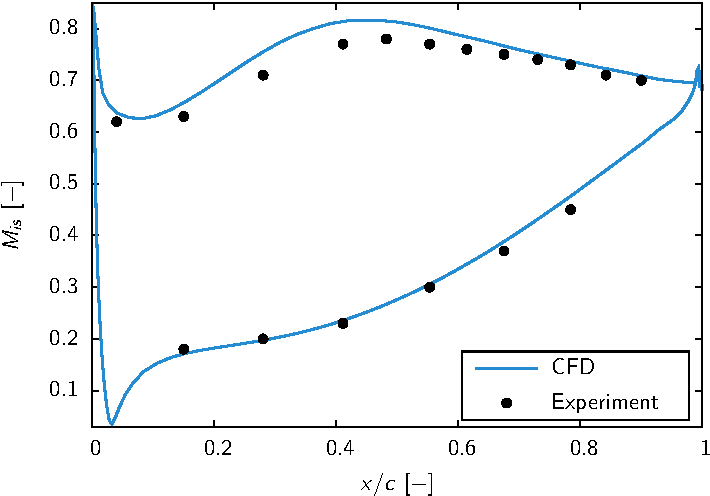
\includegraphics[height=.3\textwidth]{STCF11_RANS_SUBSONIC_PPT.pdf}}
  \subfigure[Contours]{
  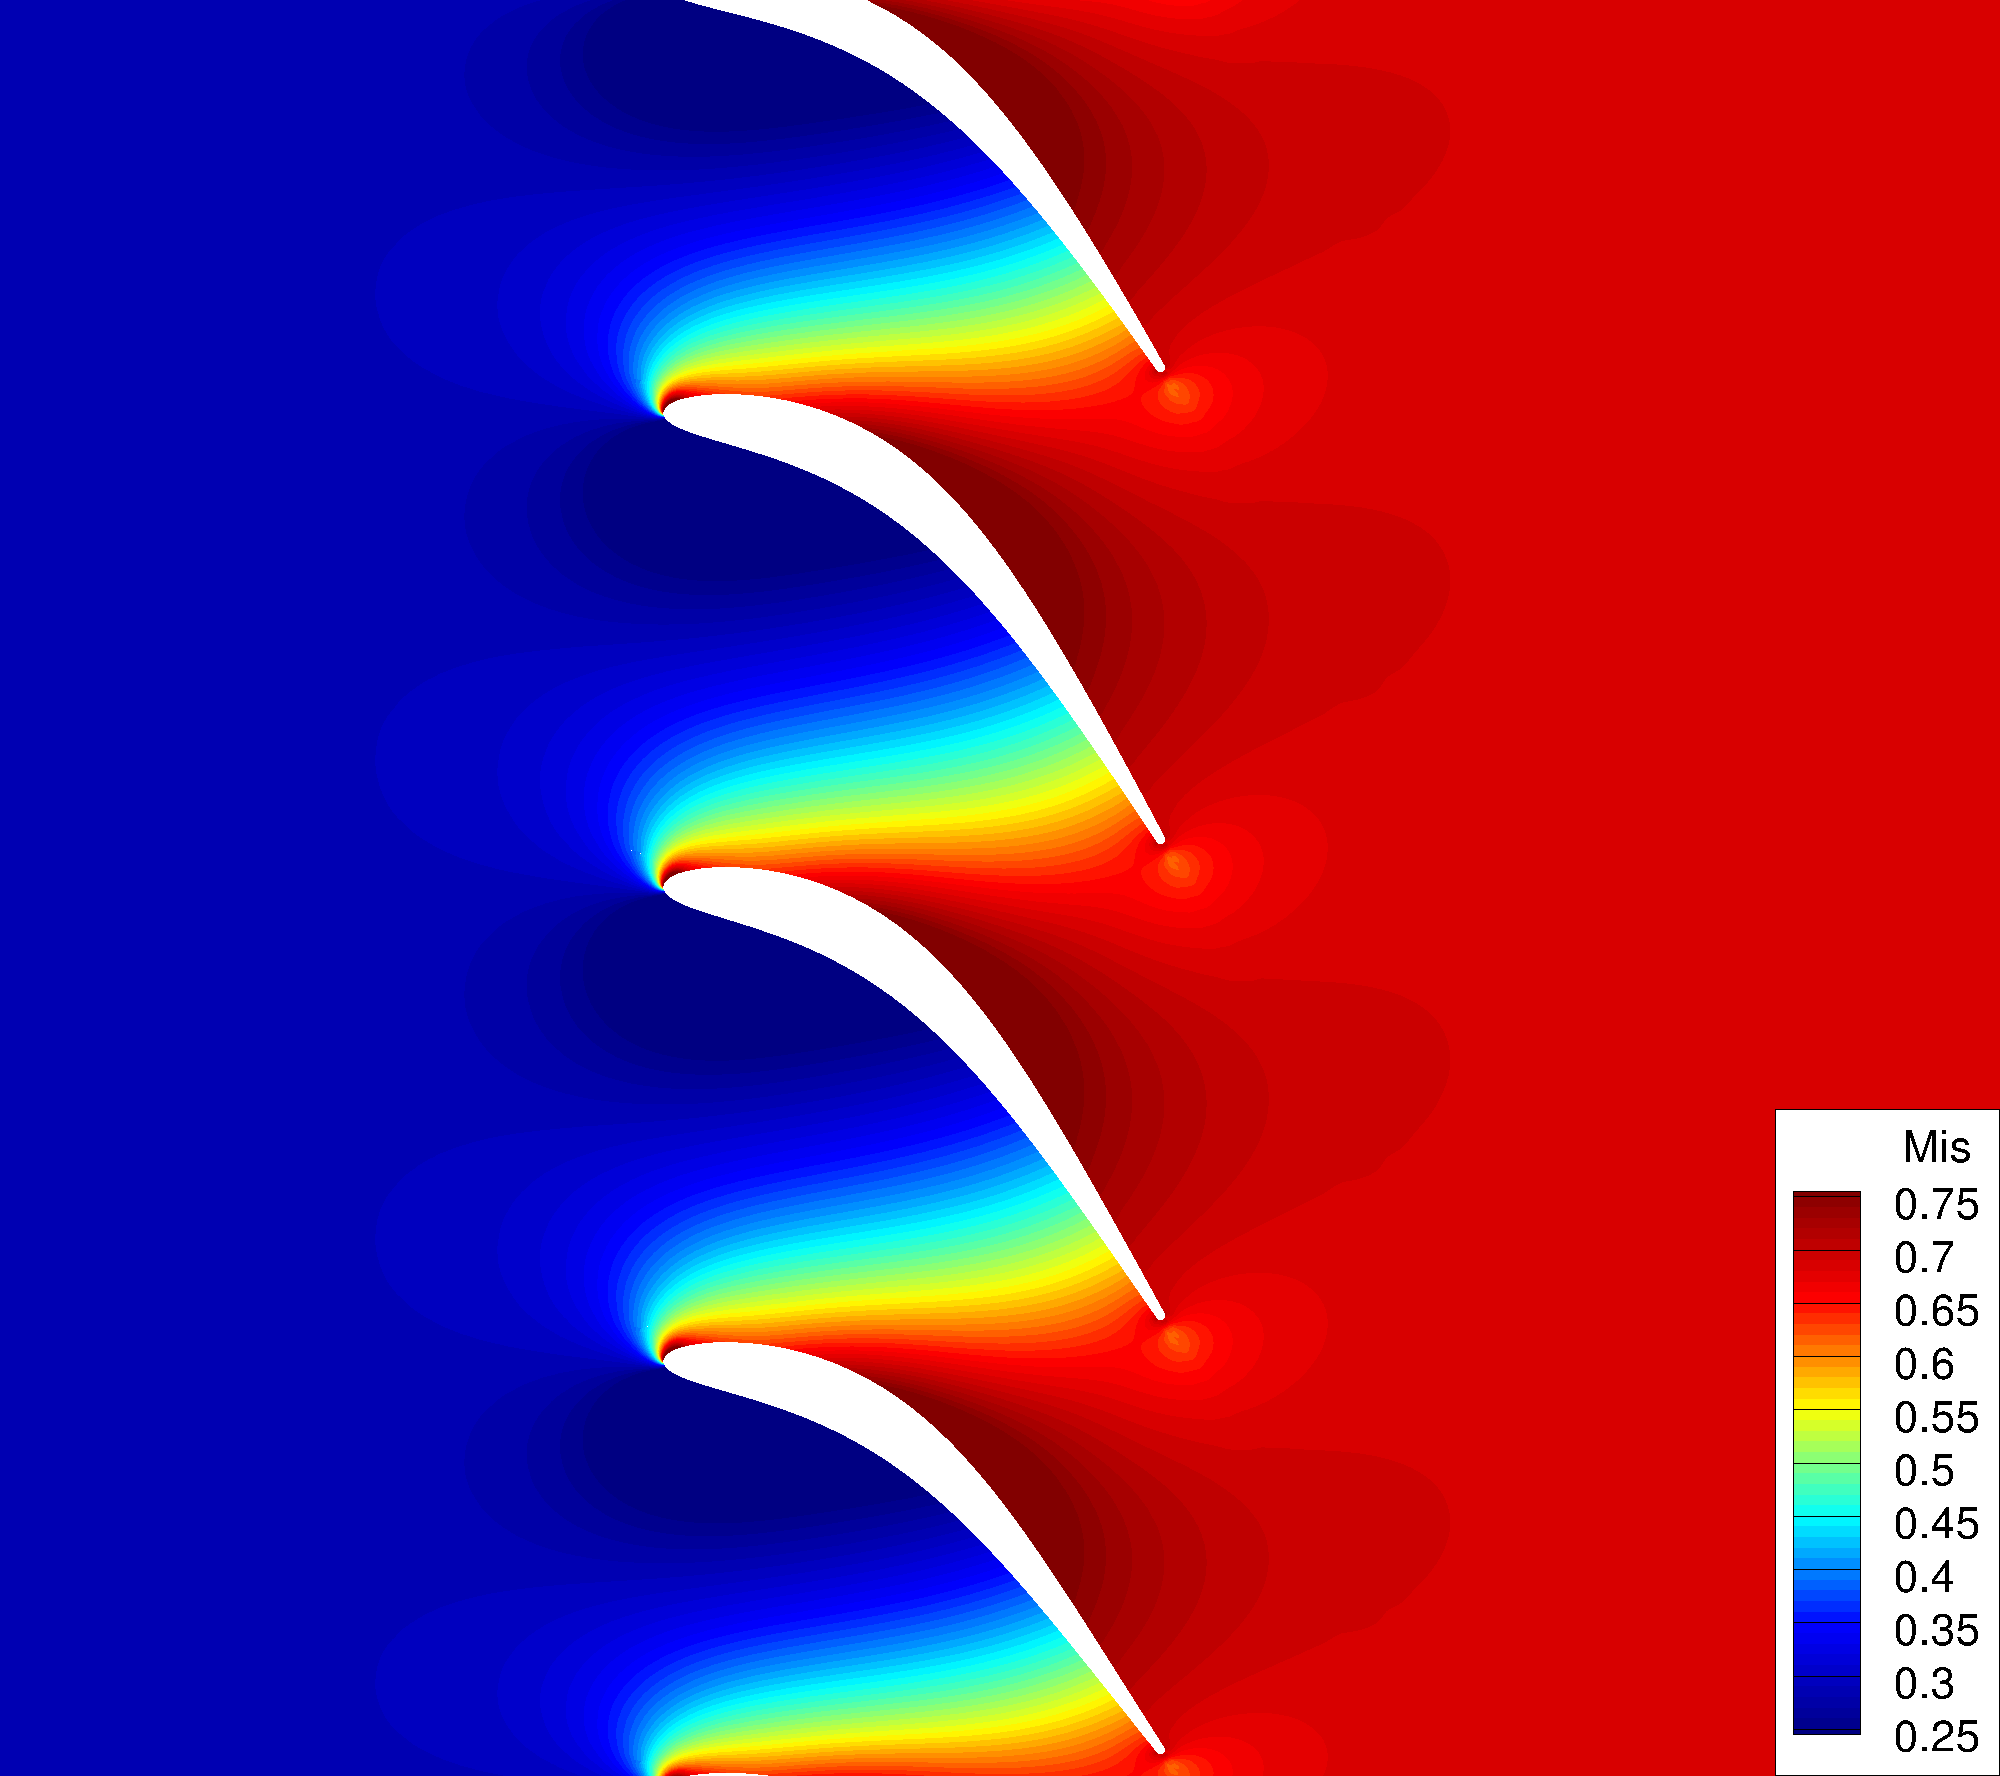
\includegraphics[height=.3\textwidth]{stcf11_subsonic.png}}
  \caption{Steady results of the isentropic Mach number, subsonic case.}
  \label{fig:stcf11_rans_subsonic}
\end{figure}

% unsteady results
The aeroelastic experimental data are compared to the present results
obtained with both the DTS and the HB approach. To explore the range
of nodal diameters with the HB method, an incremental approach is used
where each nodal diameter simulation is used to initialize the next
one.  Considering the opposite phase vibration case (the 10\textsuperscript{th} nodal diameter), 
the amplitude and the phase of the pressure coefficient are
presented in Fig.~\ref{fig:stcf11_ael_subsonic_ibpa_180_paper}.
With only one harmonic (\emph{i.e.},~three instants), the HB results
are superimposed with the DTS ones. Moreover, the numerical results are
in fair agreement with the experimental data for the
amplitude. However, for the phase, the sign change on the
suction side is predicted at about $60~\%$ of the chord, whereas the
experimental location is about 25~\%.
\begin{figure}[htb]
  \centering
  \subfigure[Amplitude]{
  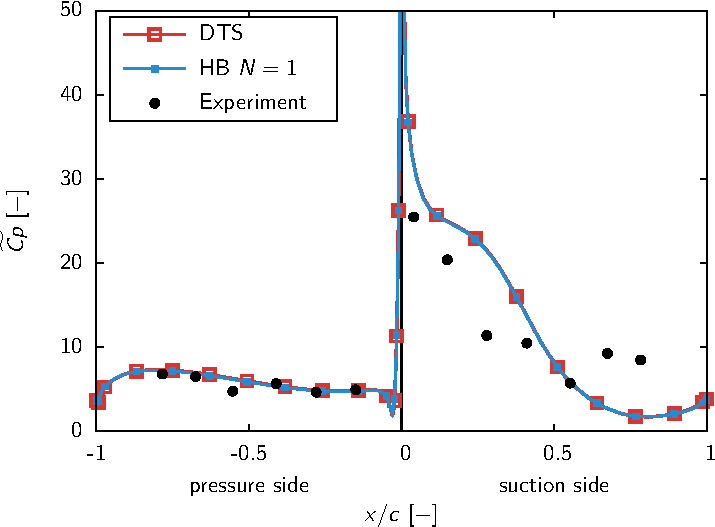
\includegraphics[width=.4\textwidth]{STCF11_AEL_SUBSONIC_IBPA_180_Cp_PPT.pdf}}
  \subfigure[Phase]{
  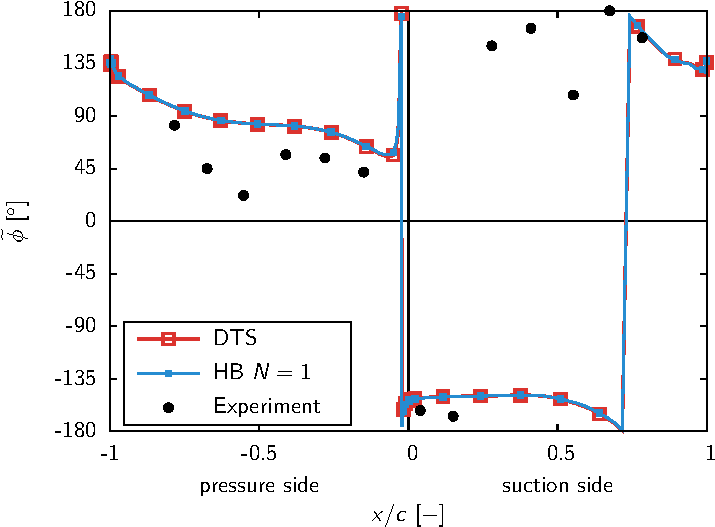
\includegraphics[width=.4\textwidth]{STCF11_AEL_SUBSONIC_IBPA_180_Phi_PPT.pdf}}
  \caption{Wall pressure harmonic analysis for an opposite phase vibration, subsonic case.}
  \label{fig:stcf11_ael_subsonic_ibpa_180_paper}
\end{figure}


The results for the  nodal  diameter $-2$ are shown
in Fig.~\ref{fig:stcf11_ael_subsonic_ibpa_324_paper}. The HB and DTS data
are superimposed, and are in fair agreement with the experiments. The
amplitude levels are well captured and the phase prediction is
slightly improved over the opposite phase case.
\begin{figure}[htb]
  \centering
  \subfigure[Amplitude]{
  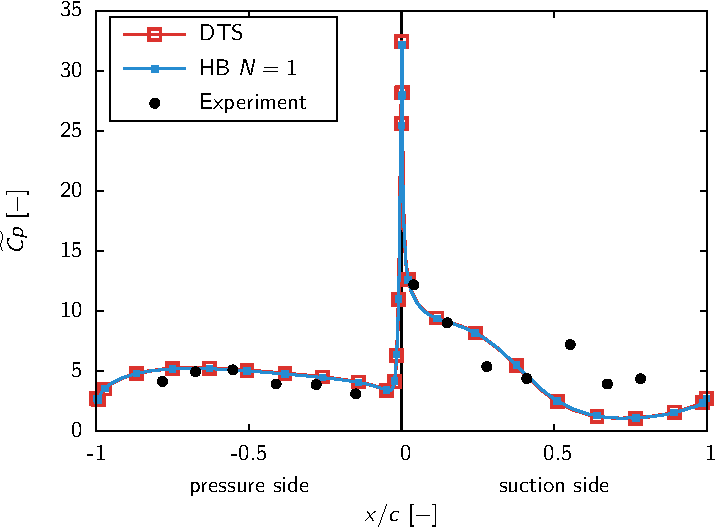
\includegraphics[width=.4\textwidth]{STCF11_AEL_SUBSONIC_IBPA_324_Cp_PPT.pdf}}
  \subfigure[Phase]{
  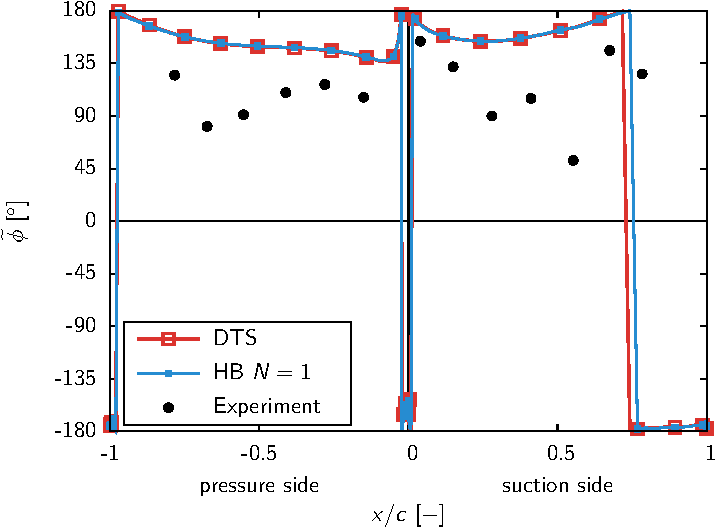
\includegraphics[width=.4\textwidth]{STCF11_AEL_SUBSONIC_IBPA_324_Phi_PPT.pdf}}
  \caption{Wall pressure harmonic analysis for afor \mbox{$n_d=-2$}, subsonic case.}
  \label{fig:stcf11_ael_subsonic_ibpa_324_paper}
\end{figure}

The damping obtained from the previous calculations is depicted 
in Fig.~\ref{fig:stcf11_subsonic_damping}.  Also plotted are the results
% from \citet{Fransson1999}, obtained with both
% potential, linear Euler, non-linear Euler and non-linear viscous codes.
from \citet{Fransson1999}, obtained with a
potential code.
% The results for all IBPAs are given for the potential code but only $\beta=180^\circ$ is provided for the other codes~\cite{Fransson1999}.
These are the only damping results for the
subsonic case known by the authors.  Since the local variations are
superimposed for the DTS and the HB approaches, so are the damping.
The present
results show similar trends and levels to those of \citet{Fransson1999}.
\begin{figure}[htb]
  \centering
  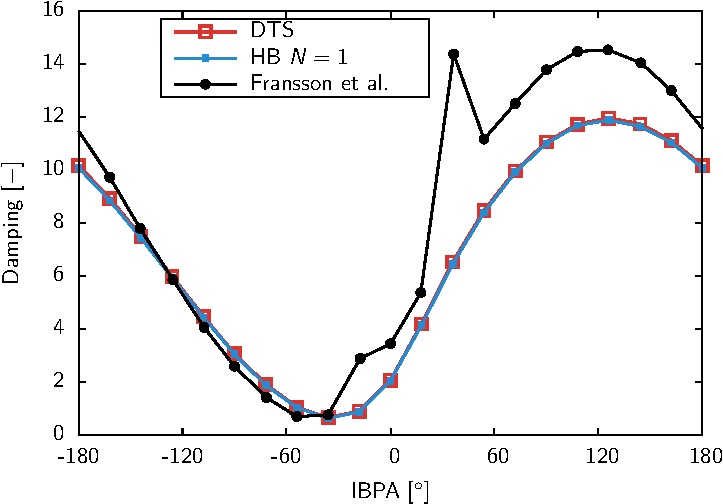
\includegraphics[width=.46\linewidth]{STCF11_SUBSONIC_DAMPING_PPT.pdf}
  \caption{Aerodynamic damping coefficient versus IBPA, subsonic case}
  \label{fig:stcf11_subsonic_damping}
\end{figure}

\section{Transonic condition}
\label{sec:stcf11_transonic}
%!TEX root = ../../../adrien_gomar_phd.tex

The outlet isentropic Mach number is $0.99$ for an inlet Mach number of $0.4$. 
This case, for which experimental uncertainties are available, 
has been largely addressed in the literature by
\citet{Sbardella2001,Duta2002,Campobasso2003,Cinnella2004} and \citet{Huang2013a}. 
This test case is challenging in terms of non-linearities as a separation bubble and a shock are present.

\paragraph{Steady results}

Steady results of the isentropic Mach number are shown in
Figure~\ref{fig:stcf11_rans_transonic}.  For this flow regime,
a small separation
bubble develops on the suction side at the leading edge.  
The flow then accelerates, followed by a shock.  
The experimental data suggests that the shock appears
sooner on the suction side than in the computations; all the results 
reported in the literature exhibit similar discrepancies (see
Refs.~\cite{Fransson1999,Sbardella2001,Duta2002,Campobasso2003,Cinnella2004,Huang2013a}). 
Otherwise, the present results are in fair agreement with experimental data.
\begin{figure}[htp]
  \centering
  \subfigure[isentropic Mach number at blade walls]{
  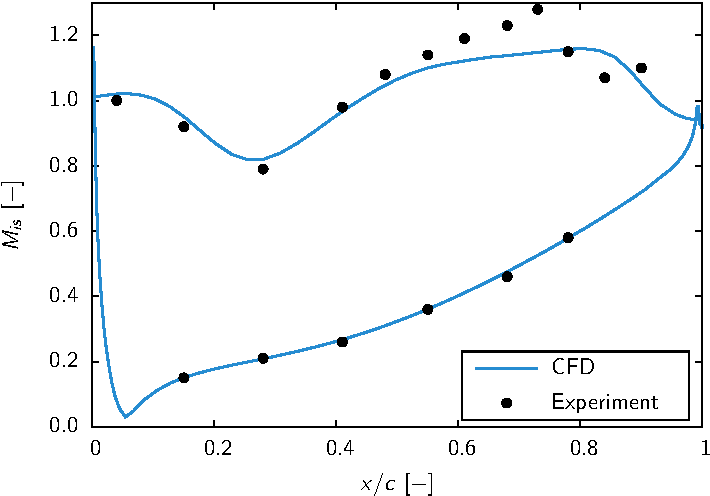
\includegraphics[height=.3\textwidth]{STCF11_RANS_TRANSONIC_PPT.pdf}}
  \subfigure[contours of the normalized static pressure with streamlines]{
  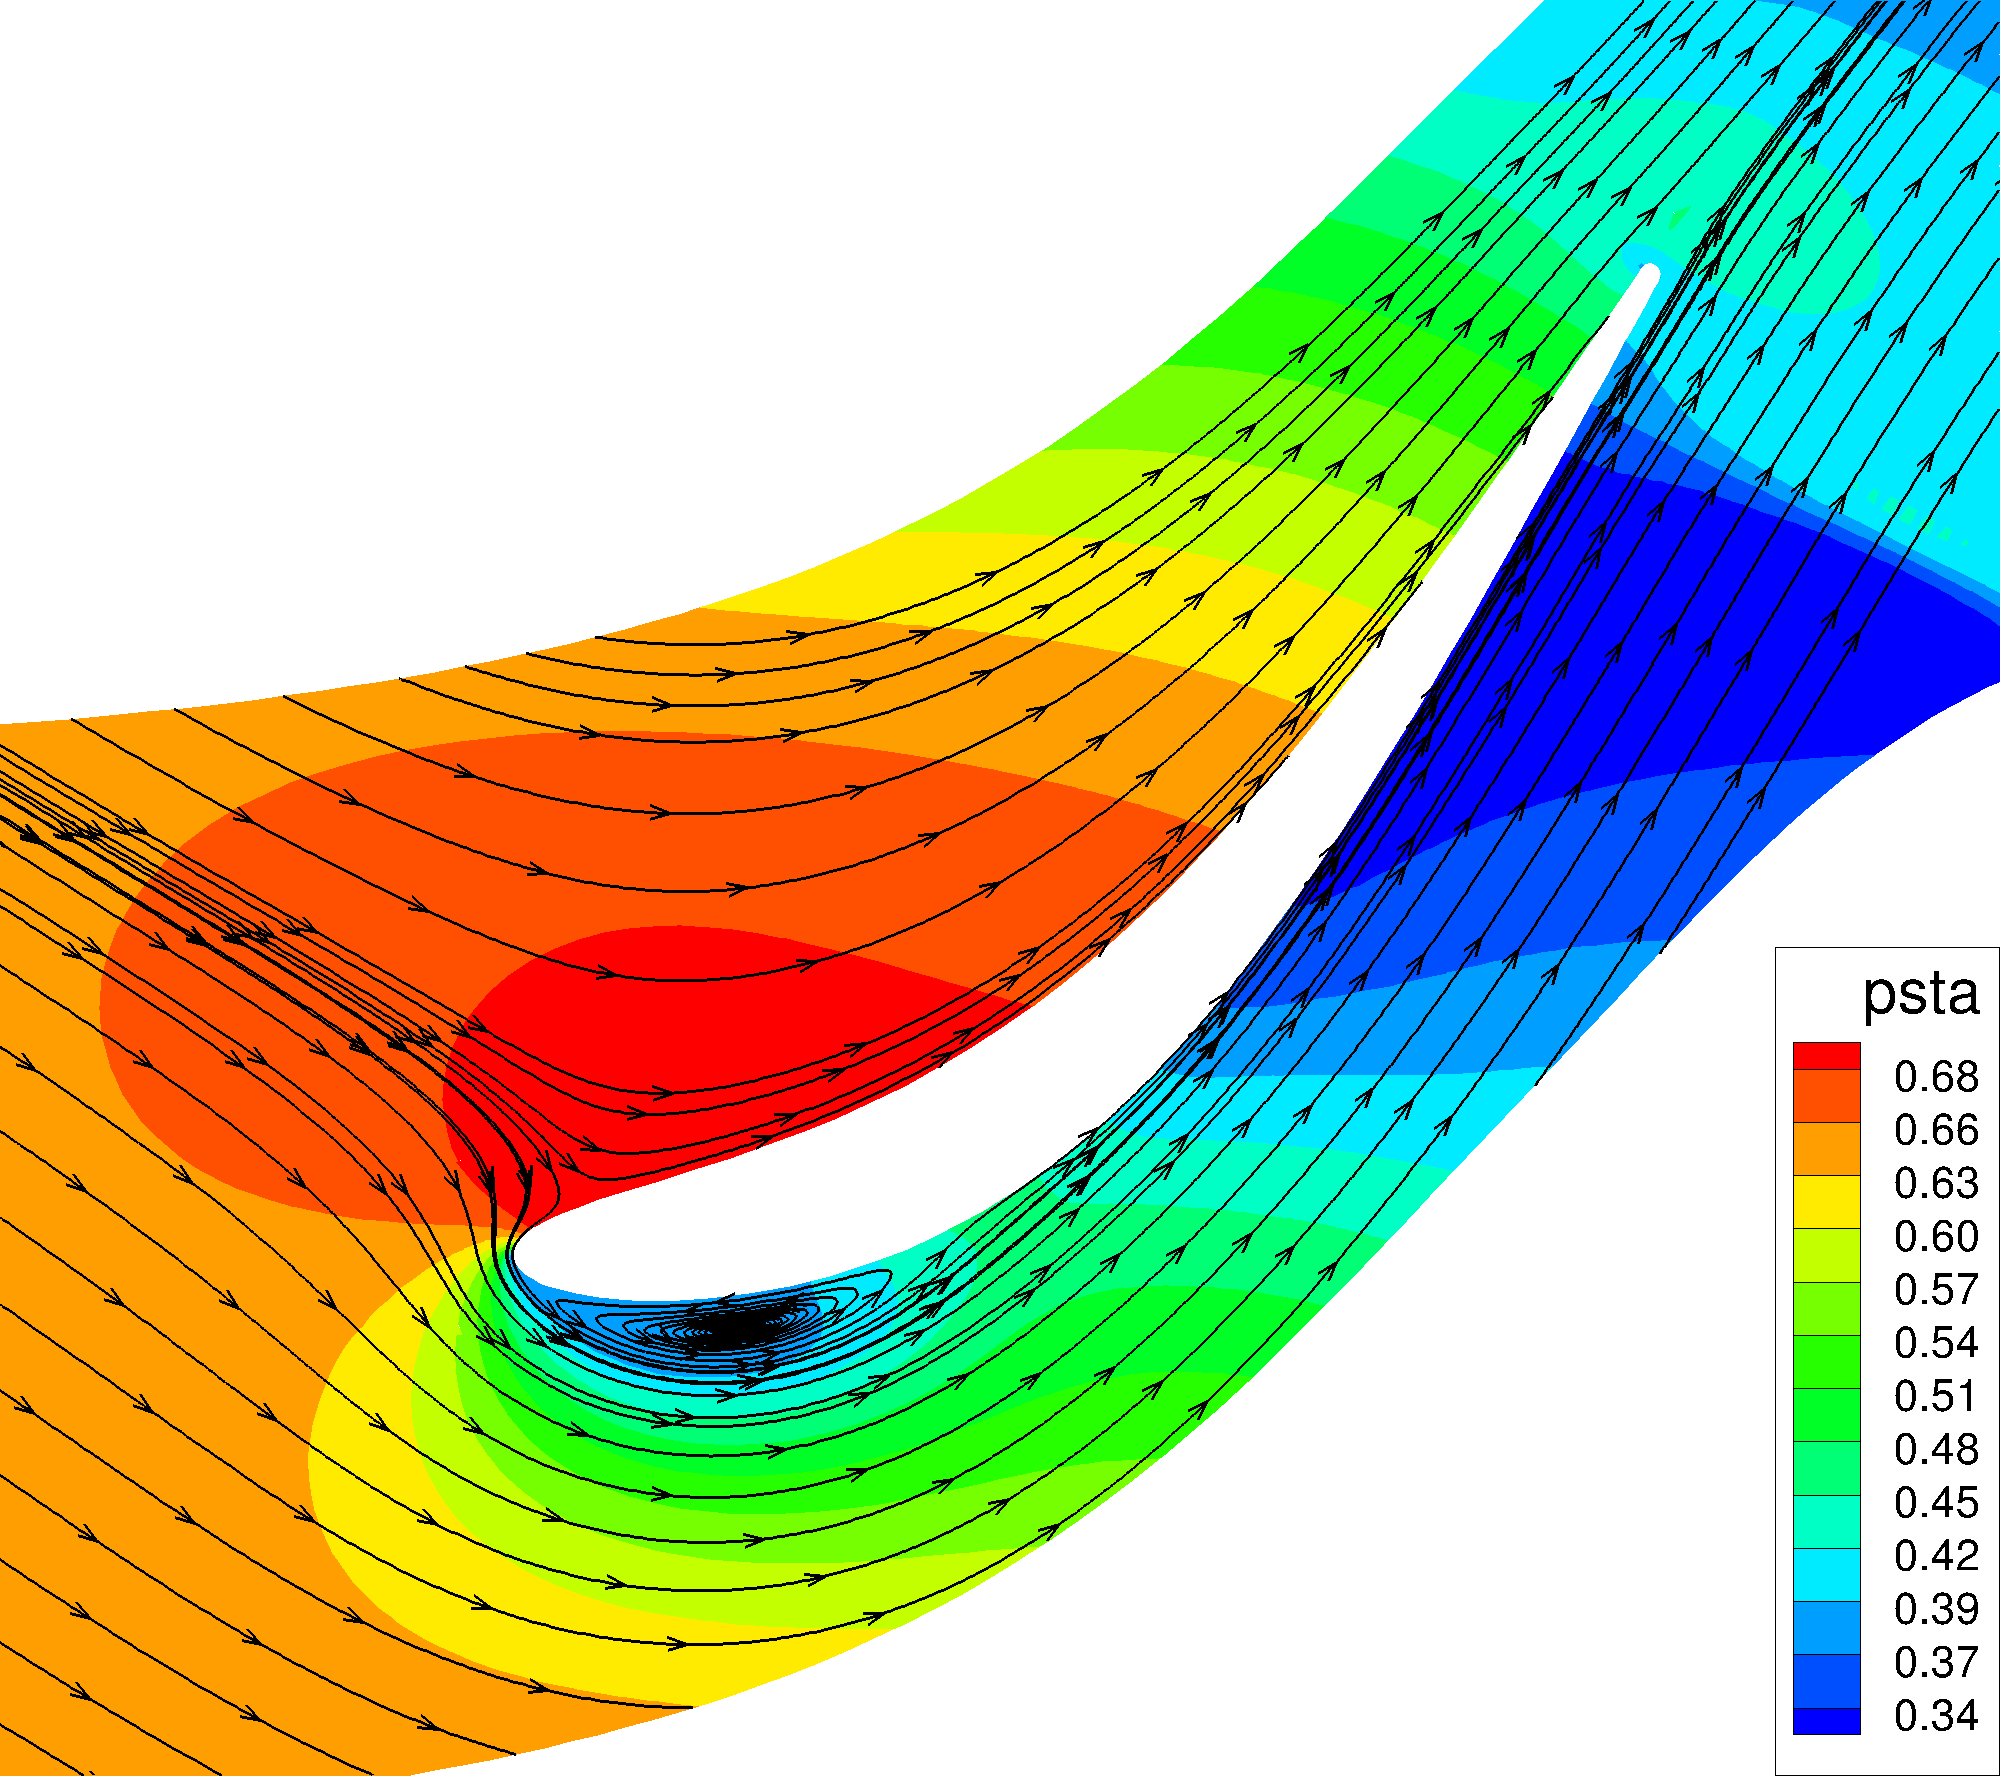
\includegraphics[height=.3\textwidth]{stcf11_transonic_local.png}}
  \caption{Steady results for the STCF~11 configuration, transonic case.}
  \label{fig:stcf11_rans_transonic}
\end{figure}

\paragraph{Aeroelastic results}

% unsteady results
The aeroelastic experimental data are compared to the present results
obtained with both the DTS and the HB approach.  
Considering the opposite phase vibration case (the 10\textsuperscript{th} nodal diameter), 
the amplitude and the
phase of the pressure coefficient are presented in
Figure~\ref{fig:stcf11_ael_transonic_ibpa_180_paper}. Also plotted are the results of
\citet{Cinnella2004}, computed with a non-linear viscous
approach using also the Spalart-Allmaras turbulence model. The present HB and the DTS
results are superimposed, which indicates that the one harmonic HB solution is able
to reproduce the unsteady non-linear effects without increasing the
number of harmonics. The results are in good agreement with
the experimental data and display the same trends as that of
\citet{Cinnella2004}. A slight discrepancy can be observed within the shock
region, where the amplitude and the phase phenomena are predicted
further than the experiments indicate.  This can be attributed to the poor
prediction of the shock position (indicated in 
Figure~\ref{fig:stcf11_rans_transonic}) and thus the poor prediction
of its interaction with the motion of the blade.
\begin{figure}[htp]
  \centering
  \subfigure[amplitude]{
  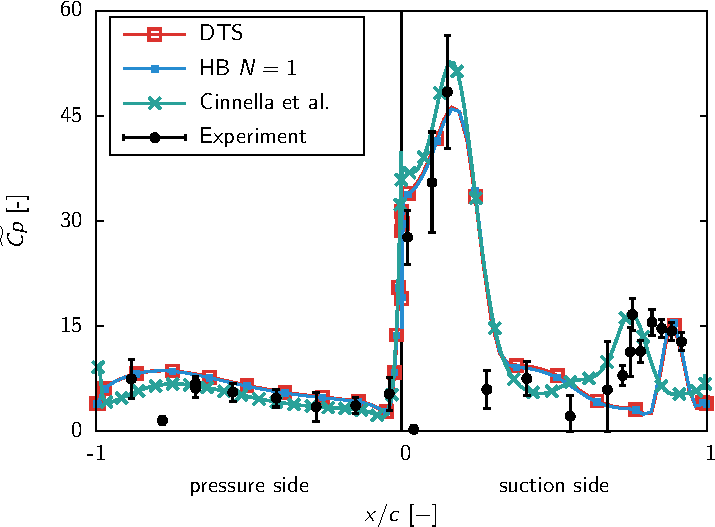
\includegraphics[width=0.45\textwidth]{STCF11_AEL_TRANSONIC_IBPA_180_Cp_ppt.pdf}}
  \subfigure[phase]{
  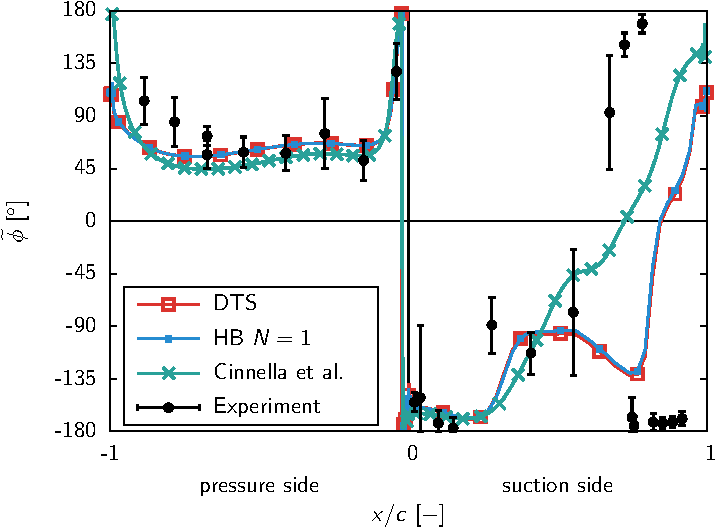
\includegraphics[width=0.45\textwidth]{STCF11_AEL_TRANSONIC_IBPA_180_Phi_ppt.pdf}}
  \caption{Wall pressure harmonic analysis for an opposite phase vibration, transonic case.}
  \label{fig:stcf11_ael_transonic_ibpa_180_paper}
\end{figure}

The results for the $-2$ nodal diameter are also shown in
Figure~\ref{fig:stcf11_ael_transonic_ibpa_324_paper}. Again,
the HB results are superimposed with the DTS ones. Moreover, these are in
good agreement with the experiments, considering the uncertainties of
the experimental data.
\begin{figure}[htp]
  \centering
  \subfigure[amplitude]{
  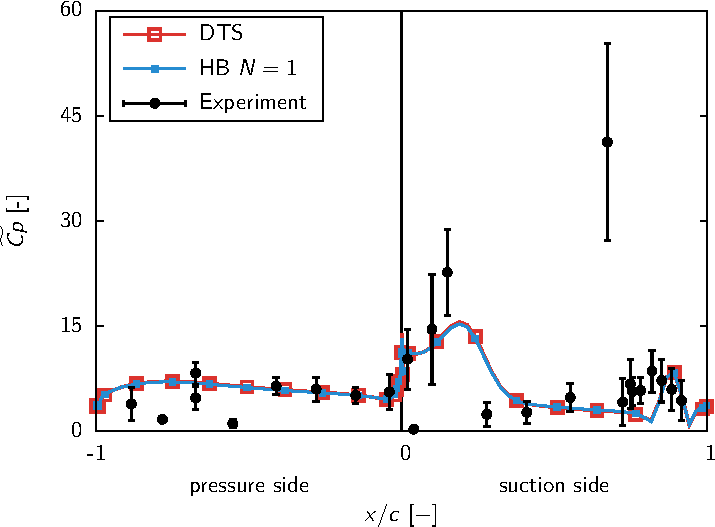
\includegraphics[width=0.45\textwidth]{STCF11_AEL_TRANSONIC_IBPA_324_Cp_ppt.pdf}}
  \subfigure[phase]{
  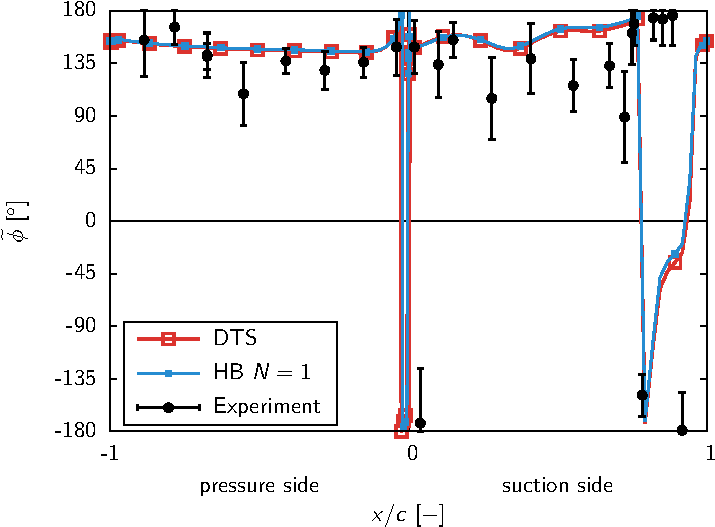
\includegraphics[width=0.45\textwidth]{STCF11_AEL_TRANSONIC_IBPA_324_Phi_ppt.pdf}}
  \caption{Wall pressure harmonic analysis for \mbox{$n_d=-2$}, transonic case.}
  \label{fig:stcf11_ael_transonic_ibpa_324_paper}
\end{figure}

Let us clarify one important thing here: 
the convergence of the harmonic balance approach depends
on the smoothness of the temporal phenomenon.
This effect can be emphasized by two 
aeroelastic computations that have been performed 
using a harmonic balance approach. 
The first one is the case of 
an airfoil with an oscillating 
flap~\cite{JDufour2009}. In this simulation, the flap is oscillating
under transonic inflow conditions, resulting in a shock swinging temporally
back and forth from the pressure side to the
suction side. As the discontinuity is
both spatial (a shock is seen on the field) and temporal
(this shock is moving with respect to time), the number
of harmonics needed to capture this phenomenon was high ($N=3$). This is
consistent with the capturing of a rectangular function
as shown in Sec.~\ref{cha:limitations_convergence}
\added{and with the results of \citet{Maple2004}, as
more than 35~harmonics are required to capture an
unsteady shock}.

Contrarily, a recent publication~\cite{Huang2013a} and the
current results on the validation
of the use of harmonic balance approach to predict
aeroelasticity damping within turbomachinery, have highlighted
different conclusions. Under the first bending mode
of the blade, the shock remains \added{almost} 
steady in the relative bending frame
of reference. As the shock
is only spatial, both authors show a convergence of the
harmonic balance approach with only $N=1$ harmonic
\added{in this region}. Thus, if the shock
structure is not evolving in time, Fourier-based time methods will not need
extra harmonics to converge, while for a temporally moving discontinuity
(which is not our case here), the number
of harmonics to converge will be higher. \added{However, a
finer mesh might draw other conclusions. In fact,
the steady results already gave a poor estimation of the
shock position (see Sec.~\ref{sec:stcf11_transonic}). Therefore,
a finer local resolution and a larger blade oscillation might
lead to different conclusions even though the idea remains.}

The damping is shown in Figure~\ref{fig:stcf11_transonic_damping} for
the transonic case. Also plotted are the results from
\citet{Fransson1999} (potential code), and 
from \citet{Cinnella2004} (RANS code). The scattering is much more severe
than for the subsonic case. The trends obtained with the RANS 
approaches are similar, but the discrepancies in terms of
levels are significant.
Recently, \citet{Vogt2011} reported similar discrepancies 
for damping predictions of subsonic and transonic cascades, 
showing that the damping can be significantly affected by 
small local changes in the amplitude or the phase.
\begin{figure}[htp]
  \centering
  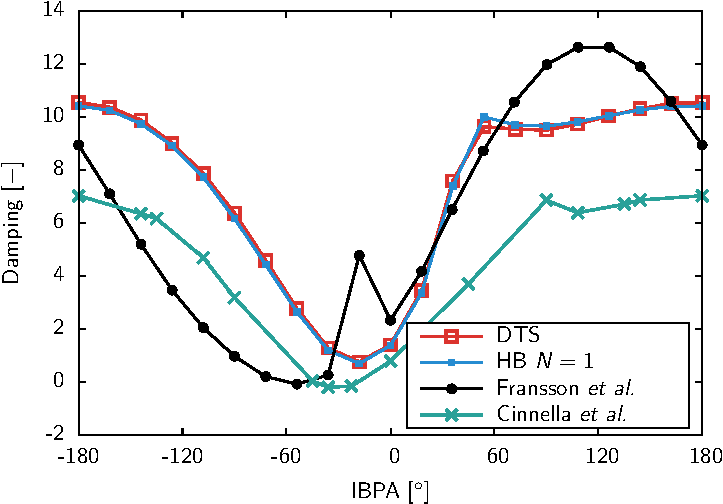
\includegraphics[width=.4\linewidth]{STCF11_TRANSONIC_DAMPING_PPT.pdf}
  \caption{Aerodynamic damping coefficient versus IBPA, transonic case.}
  \label{fig:stcf11_transonic_damping}
\end{figure}

In terms of computational efficiency, the HB method is 7 times faster
than the DTS for all the IBPAs which is very good considering 
that the DTS computations
were done using chorochronic boundary conditions which already
provides computational savings compared to a
full $360^\circ$ simulation. Actually the $N=1$ harmonic
balance computation is 3 times more expensive than a
steady RANS simulation, which is consistent with the
theoretical cost estimation (see Sec.~\ref{sec:sm_hb_cost}).


\chconclu{The use of harmonic balance approach
to compute turbomachinery aeroelasticity has been validated
against a well-known experimental test case. The results
are in good agreement with the experimental data and with
different numerical approaches.
The harmonic balance approach
has shown that with only one harmonic, the damping curve
is retrieved compared to a classical time-marching scheme.
The speed-up obtained is seven. This give us faith to
apply the current approach to more demanding aeroelastic
computations, namely contra-rotating open rotor
aeroelasticity.}
